In this section, we first present the \PICI implementation and evaluate its performance and the resulting soundness improvement~(Section~\ref{subsec:pici_impl}).
For comprehensiveness, we then also  verify that not only the CPU, but also the rest of the platform complies with its own contract terms, i.e., that a platform will not propagate more taint than what the contract stipulates~(Section~\ref{subsec:pici_platform}).

\para{Evaluation setup}
We execute the performance evaluations on a server equipped with an Intel Xeon E5-2667 CPU with 256\,GB RAM.
We use the 2-stage Sodor RISC-V CPU~\cite{sodor}, which is a simple CPU commonly used in constant-time verification benchmarks~\cite{wang2023specification,tan2025contractshadowlogic}.

% \para{The problem with a CPU in isolation}
% We now show that techniques can be unsound because the SoC integration is not considered.
% In particular, we show that \ucfi~\cite{ceesay2024mucfi} and VeloCT~\cite{dinesh2025h} call instructions safe, but these instructions are not safe when the CPU is integrated into a platform that contains a cache.
% We execute \ucfi and VeloCT on the 2-stage Sodor RISC-V CPU~\cite{sodor} (commit \texttt{32d49f9}) and ask whether loads and stores are safe instructions, which the two techniques answer positively because they do not consider reentrant information flows.

% We introduce a simple SoC architecture composed of a Sodor CPU, a set-associative cache and memory as depicted in Figure~\ref{fig:simple_soc}.
% We mount a cache attack on the SoC, where we measure the timing differences in cache access patterns when secret data is used as an address, and we obtain different timing results depending on whether the secret data causes a hit or a miss in the cache.
% As a result of this experiment, we indeed observe differences in the timing of the memory accesses between a hit and a miss using exclusively instructions that \ucfi and VeloCT considers safe.
% This demonstrates that instructions that were considered safe by some techniques are not necessarily safe when the CPU is integrated into a platform that contains a cache.
% This justifies the need for \pics, which model an upper bound for reentrant information flows through the platform.

\subsection{\PICI implementation}
\label{subsec:pici_impl}

The limited interface between the CPU and the platform makes the \PICIs simple, as earlier illustrated in Figure~\ref{fig:pic_instrum_taints} and Figure~\ref{fig:pic_instrum_miter}.
We implement a Yosys synthesizer pass~\cite{wolf2013yosys} that instruments a CPU that is either instrumented with taint tracking logic such as GLIFT~\cite{tiwari2009complete} or CellIFT~\cite{solt2022cellift}, or part of a miter construct.
The synthesizer pass takes as input a Verilog description of the CPU under test in one of these two configurations (instrumented for taint tracking or in a miter) and outputs a Verilog design instrumented with the \PICI.
In addition to the CPU's Verilog description, the synthesizer pass takes a conditional contract as input, similar to the contracts presented in Section~\ref{sec:reentrant}, and takes a machine-readable description of the CPU's interface ports.
% The \PICI synthesizer pass is made of around 500 lines of C++ code.
% \fls{TODO: Give an example contract in appendix and of the CPU interface ports file.}

\begin{figure}[t]
    \begin{center}
    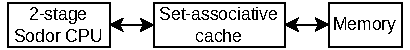
\includegraphics[width=0.80\columnwidth]{figures/simple_soc/simple_soc.pdf}
    \end{center}
    \vspace*{-1em}
    \caption{\label{fig:simple_soc} Simple SoC architecture with a CPU, a set-associative cache and memory.}
    \vspace*{-1.4em}
\end{figure}

\begin{table}[t]
    \vspace*{1.2em}
    \centering
    \caption{Verification results for the original Sodor (O) design, for \PICI-instrumented (Equation~\ref{dict:contract_cache_nointerrupt}) Sodor (P). Results are "pass" if memory instructions are considered safe with regard to all their operands (and in particular with regard to the address).
    \textcolor{red}{TODO Add results for no-violation scenarios.}
    }
    \vspace*{-.4em}
    \small
    \begin{tabular}{|l|c|c|c|c|}
        \hline
        \rowcolor{gray!20} % Color for the table header
        & \textbf{\ucfi} & \textbf{VeloCT} \\
        \hline
        Time  (O) & 8\,min & 1\,min \\
        \hline
        Result (O) & Pass \gcheck & Pass \gcheck \\
        \hline
        Time (P)  & 10\,min & 1\,min \\
        \hline
        Result (P) & Fail \rcross & Fail \rcross \\
        \hline
    \end{tabular}
    \vspace*{-.4em}
    \label{tab:verif_results_simple_soc}
\end{table}


\subsection{Soundness improvement with \PICI}
\label{subsec:pici_platform}

We have shown that the security guarantees provided by \ucfi and VeloCT may not hold when the CPU is integrated into a platform that contains caches or other elements that have an address-dependent timing, for example described by the contract defined in Equation~\ref{dict:contract_cache_nointerrupt}.
% Sodor is a simple CPU core that belongs to LeaVe's and CSL's constant-time verification testbench.
% \fls{Abrupt introduction of Sodor.}
We first verified Sodor with \ucfi and VeloCT (ConjunCT is not open-source but is superseded by VeloCT).
We now instrument Sodor with the \PICI and verify it again with the same tools.
We report the verification results, as well as the time taken by each tool to formulate a proof in Table~\ref{tab:verif_results_simple_soc}.
We observe that the \PICI indeed can correct the unsoundness of \ucfi and VeloCT with regard to the platform integration such as cache side channels.
As a result, the \PICI automatically transforms the verification of a CPU in isolation into a verification of a CPU in a contract-compliant platform.

% \begin{table}[t]
%     \centering
%     \caption{Verification of the compliance of platforms to \PICI. SimpleSoC is depicted in Figure~\ref{fig:simple_soc}, exempt of Sodor.}
%     \small
%     \begin{tabular}{|l|c|c|}
%         \hline
%         \rowcolor{gray!20} % Color for the table header
%         & \textbf{SimpleSoC} & \textbf{Caliptra} \\
%         \hline
%         Time  (Contract A) & \textcolor{red}{TODO Measure} & \textcolor{red}{TODO Measure} \\
%         \hline
%         Result (Contract A) & Pass & Fail \\
%         \hline
%         Time  (Contract B) & \textcolor{red}{TODO Measure} & \textcolor{red}{TODO Measure} \\
%         \hline
%         Result (Contract B) & Pass & Pass \\
%         \hline
%         Time  (Contract C) & \textcolor{red}{TODO Measure} & \textcolor{red}{TODO Measure} \\
%         \hline
%         Result (Contract C) & Fail & Pass \\
%         \hline
%     \end{tabular}
%     \label{tab:verif_platform_compliance_results}
% \end{table}

\begin{table}[t]
    \centering
    \caption{Verification of the compliance of platforms to \PICI.}
    \small
    \begin{tabular}{|r|c|c|c|}
        \hline
        \rowcolor{gray!20} % Color for the table header
        \textbf{Contract} & \texttt{nocache} & \texttt{cache} & \texttt{interrupt} \\
        \hline
        A & Pass \gcheck & Fail \rcross & Fail \rcross \\
        \hline
        B & Pass \gcheck & Pass \gcheck & Fail \rcross \\
        \hline
        C & Pass \gcheck & Pass \gcheck & Pass \gcheck \\
        \hline
        D & Pass \gcheck & Pass \gcheck & Fail \rcross \\
        \hline
    \end{tabular}
    \label{tab:verif_platform_compliance_results}
\end{table}


\para{Platform verification}
Finally, we verify the compliance of the platform with the \pic.
Because these contracts specify a form of non-interference, they can be verified conveniently with miter constructs, similar to how most techniques verify constant-time properties for CPUs~\cite{dinesh2024conjunct,dinesh2025h,wang2023specification,tan2025contractshadowlogic}.
We verify three platforms.
The \texttt{cache} platform is a simple SoC architecture composed of a CPU, a set-associative cache and memory, as depicted in Figure~\ref{fig:simple_soc}.
The \texttt{nocache} platform is like the \texttt{cache} platform, but the cache is removed, connecting the CPU directly to the memory, which is modeled as having no address-dependent latency.
The \texttt{interrupt} platform is like the \texttt{cache} platform, but also adds an uncached interrupt controller at the address \texttt{0x1000}, which generates an interrupt signal when a non-zero value is written to this address.
For each of these platforms, we verify Contract A that we define as in Equation~\ref{dict:contract_cache_nointerrupt}, Contract B that we define as in Equation~\ref{dict:contract_cache_interrupt}, Contract C that we define as in Equation~\ref{dict:contract_cache_interrupt_addressdependent} where we constrain \texttt{periph\_range} to be \texttt{0x1000} to \texttt{0x1000}, and Contract D that is like Contract C but with a \texttt{periph\_range} of \texttt{0x2000} to \texttt{0x2FFF}.
% \fls{TODO Check the mem range for Caliptra.}
% \fls{TODO Say that the caliptra contract proves that the ICCM and DCCM indeed do not have timing side channels, as expected}
We construct miters whose designs under test is the platform seen from the CPU's perspective, i.e., whose inputs are the outputs of the CPU, and whose outputs are the inputs of the CPU.
Note that the CPU itself is not part of this miter.
To verify, for example, the last arrow of Equation~\ref{dict:contract_cache_interrupt_addressdependent}, we enforce all inputs of the miter to be identical between the two sides of the miter except for the \texttt{mem\_wdata} input, and we additionally constrain the \texttt{mem\_addr} input, identical between the two sides of the miter, not to be in the \texttt{periph\_range} range.
We then verify that only \texttt{mem\_rdata} can be affected by changes to \texttt{mem\_wdata} by \texttt{xor}'ing the outputs of \texttt{mem\_gnt} for the two copies of the platform in the miter together and expressing a SAT formula on this signal, which should never be set.
Table~\ref{tab:verif_platform_compliance_results} summarizes the verification results obtained with Cadence Jaspergold for the different platforms.
The total duration of the experiment does not exceed one minute.
\fls{TODO report the simulation results for no violation found.}

\fls{Takeaway box: Given a platform specification, \PICI includes reentrant information flows in the verification of constant-time properties, even if the underlying verification technique initially did not account for them}
% \takeawayBox{Given a platform specification, \PICI includes reentrant information flows in the verification of constant-time properties, even if the underlying verification technique initially did not account for them.}
